\section{Cài đặt và tái lập}
\label{sec:repro}
Môi trường dùng Python 3.11, quản lý bằng \code{uv} (\code{pyproject.toml}, \code{uv.lock}), với PyTorch, PyTorch Geometric, open\_clip và FAISS. Các lệnh chính để chạy lại pipeline cấp độ 1 trên Visual Genome:

{\footnotesize\ttfamily\raggedright
uv sync --group ml --group graph\\
uv run python scripts/make\_splits.py --config configs/splits\_visual\_genome.yaml\\
uv run python scripts/evaluate\_clip.py --config configs/clip\_vg.yaml --seed <k>\\
uv run python scripts/build\_graph.py --config configs/graph\_vg\_clip\_topk.yaml\\
uv run python scripts/train\_graph\_rerank.py --config configs/clip\_graph\_vg\_lr1e4.yaml --seed <k>\\
uv run python scripts/evaluate\_graph\_rerank.py --config configs/clip\_graph\_vg\_lr1e4.yaml --seed <k>\\
uv run python scripts/summarize\_runs.py\\
uv run python scripts/explain.py --config configs/explain\_vg.yaml\par}

\smallskip
Mỗi lần chạy ghi lại \code{config.yaml}, \code{metrics.json} và \code{env.json} (commit, phiên bản thư viện); bản sao của các lần chạy đã báo cáo nằm trong \code{results/records/}. Phần MMKG chạy bằng \code{scripts/make\_mmkg\_queries.py}, \code{scripts/evaluate\_mmkg\_transfer.py} với cấu hình \code{configs/mmkg\_vi\_transfer.yaml}. Phần Flickr30k dùng notebook \code{notebooks/20\_kaggle\_graph\_pipeline.ipynb} với \code{DATASET = "flickr30k"}.

Mỗi quyết định thiết kế quan trọng được ghi thành một ADR (architecture decision record) trước khi chạy thí nghiệm liên quan; Bảng~\ref{tab:adr} liệt kê các ADR chính.
\begin{table}[t]
\centering
\caption{Các quyết định thiết kế (ADR) chính}
\label{tab:adr}
\footnotesize
\setlength{\tabcolsep}{3pt}
\begin{tabular}{@{}l p{6.4cm}@{}}
\toprule
\textbf{ADR} & \textbf{Nội dung} \\
\midrule
0015 & Định dạng MMKG tiếng Việt và data card \\
0016 & Giải thích trung thực, tính từ chính cơ chế xếp hạng \\
0040 & Chọn Visual Genome và Flickr30k \\
0042 & Chia tập cố định cho Visual Genome, gom ảnh trùng \\
0043 & Giao thức đánh giá: mọi ảnh cùng câu đều là đáp án \\
0045--0046 & Đồ thị ảnh--khái niệm, cạnh CLIP top-$k$ cho mọi tập \\
0047 & Quy trình huấn luyện, chọn $\alpha$, chạy test một lần \\
0048 & Cạnh đồng xuất hiện đếm trên train, GraphSAGE hai lớp \\
0049 & Giao thức v2: nDCG, ảnh $\to$ văn bản, nhóm truy vấn \\
0050 & Flickr30k: chạy lại pipeline, chỉ đổi dữ liệu; miền di sản cho MMKG \\
0051 & G-Retriever: chọn đồ thị con PCST để xếp hạng lại \\
0052 & Lưu dữ liệu thô (snapshot) và duyệt riêng cho MMKG \\
0053 & Đánh giá chuyển giao sang MMKG, không huấn luyện lại \\
0054 & Đánh giá giải thích định lượng trên MMKG \\
0056 & G-Retriever trên Flickr30k: dùng lại cạnh đồng xuất hiện của Visual Genome \\
0057 & Truy vấn gián tiếp mô tả khái niệm bị giấu qua ConceptNet \\
0058 & Bộ truy vấn KG do một thành viên duyệt \\
\bottomrule
\end{tabular}
\end{table}

\section{Demo}
\label{sec:demo}
\begin{figure*}[t]
\centering
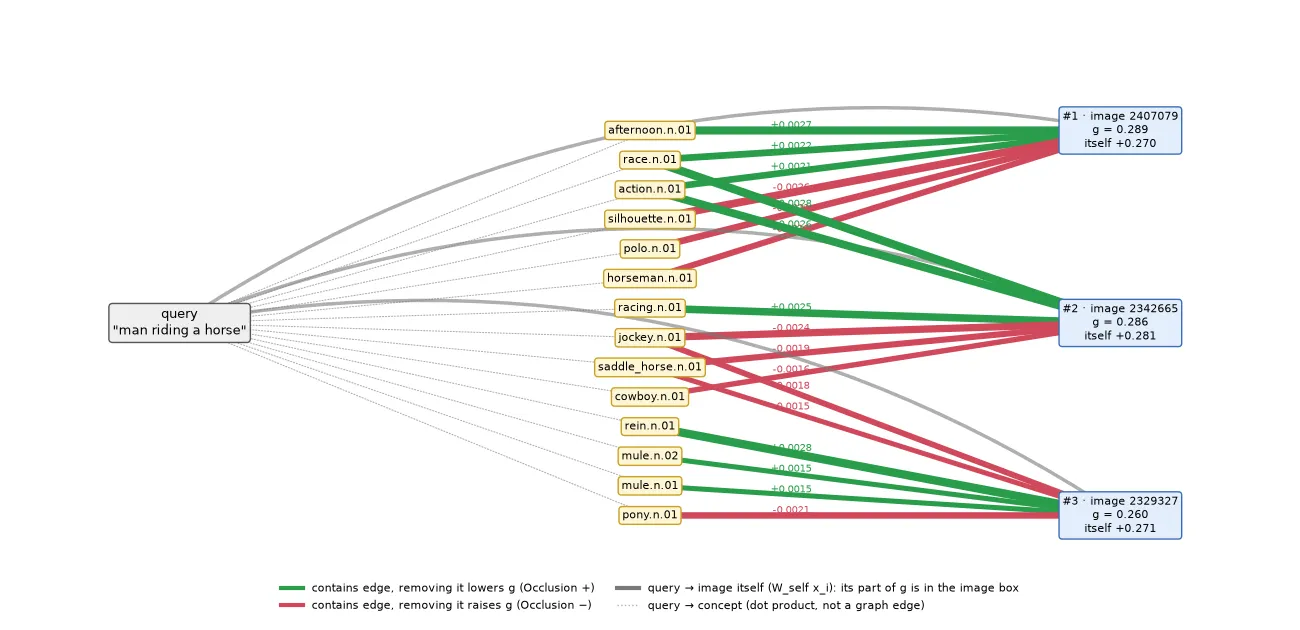
\includegraphics[width=0.8\textwidth]{query_path.png}
\caption{Giao diện demo cho truy vấn ``man riding a horse'': top-3 ảnh val và đường đi truy vấn $\to$ khái niệm $\to$ ảnh. Cạnh xanh là cạnh mà khi xóa thì điểm $g$ giảm; cạnh đỏ là cạnh kéo ảnh xuống. Ô ảnh ghi phần điểm đến từ chính ảnh ($W_{\text{self}}x_i$).}
\label{fig:demo}
\end{figure*}

\begin{figure}[t]
\centering
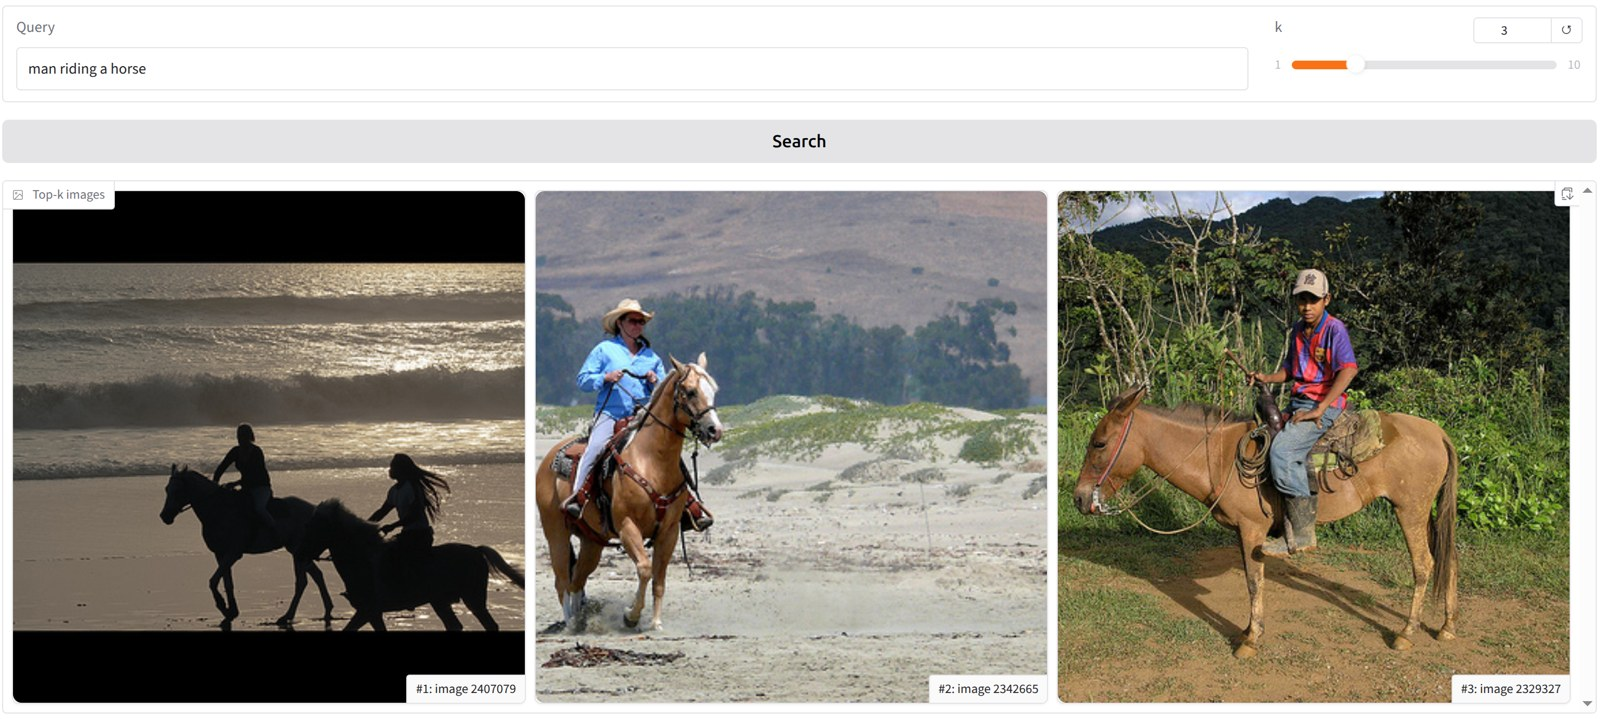
\includegraphics[width=\linewidth]{query_result.jpg}
\caption{Kết quả top-3 của demo cho truy vấn ``man riding a horse'' trên tập val Visual Genome.}
\label{fig:demo-result}
\end{figure}

Ứng dụng demo viết bằng Gradio (\code{app/gradio\_app.py}) nhận một câu truy vấn, trả về top-$k$ ảnh val (Hình~\ref{fig:demo-result}) và vẽ, cho từng ảnh, các cạnh \code{contains} đã tạo nên điểm đồ thị cùng đóng góp Occlusion có dấu của từng cạnh (Hình~\ref{fig:demo}). Giao diện chỉ gọi các hàm trong thư viện \code{src/mmxai/} của dự án, không chứa logic riêng, nên những gì hiển thị đúng là mô hình đã báo cáo. Ví dụ trong hình cho thấy cả những cạnh hợp nghĩa (\code{race}, \code{racing}, \code{rein}) lẫn những cạnh có đóng góp âm (\code{polo}, \code{jockey}). Demo chạy được trên máy không có GPU; hướng dẫn cài đặt nằm trong \code{app/README.md}.

\section{Thảo luận và hạn chế}
\label{sec:discussion}
\textit{Vai trò của đối chứng không đồ thị.} Nếu thiếu đối chứng này, toàn bộ mức tăng 19\% trên Visual Genome sẽ bị gán nhầm cho đồ thị. Kết luận ``phần lớn mức tăng đến từ phép chiếu học được'' lặp lại trên ba bộ dữ liệu (Visual Genome, Flickr30k, MMKG) và với cả G-Retriever. Đồ thị thật tốt hơn đồ thị xáo trên Visual Genome và Flickr30k, nhưng chỉ trên Visual Genome mô hình có đồ thị mới cao hơn mô hình không đồ thị; trên Flickr30k và MMKG thì không.

\textit{Thông tin trong đồ thị.} Cạnh \code{contains} được suy ra từ chính CLIP (16 khái niệm gần nhất), không có quan hệ giữa các đối tượng trong scene graph và chưa dùng ConceptNet. Lựa chọn này giúp hệ thống chạy được với ảnh chưa gán nhãn và tránh rò rỉ, nhưng khiến đồ thị mang ít thông tin mới so với những gì CLIP đã biết. Đây có lẽ là lý do chính khiến đồ thị chỉ giúp ở các truy vấn chung chung. Ngoài ra, cạnh ở mức cả ảnh không khớp với truy vấn mô tả một vùng nhỏ của Visual Genome.

\textit{Trọng số kết hợp.} Trên Visual Genome, $\alpha \approx 0$ khiến điểm cuối gần như chỉ còn nhánh học được, và các trường hợp thất bại lớn (hạng của ảnh đúng giảm từ 7--15 xuống 92--100) cho thấy một giá trị $\alpha$ chung cho mọi truy vấn là chưa phù hợp.

\textit{Giới hạn thống kê.} Mỗi thí nghiệm có 3 seed và chỉ có một bản xáo; t và $p$ tính theo seed chỉ mang tính mô tả. Nhóm chưa có kiểm định theo truy vấn. Recall là cận dưới vì mỗi ảnh chỉ xét 5 câu, MRR bị cắt ở 100, và hai câu khác chữ nhưng cùng nghĩa (``a man'', ``man'') vẫn được tính là khác nhau.

\textit{Giới hạn của MMKG.} Truy vấn được sinh bằng mẫu câu cố định, chưa có câu tự nhiên do người viết; mỗi nhóm chỉ có 35--80 câu; 2/158 câu gián tiếp vẫn để lộ tên hiện vật qua tên của thực thể đích. Nhóm chưa chạy ablation bỏ hoặc xáo bộ ba. Muốn chuyển ngôn ngữ thật sự, cần một bộ mã hóa văn bản đa ngôn ngữ; khi đó không gian vectơ thay đổi và phải huấn luyện lại GNN.

\textit{Phần chưa hoàn thành.} Bộ 38 truy vấn trực tiếp và gián tiếp trên test Visual Genome đã được xây, duyệt và chấm cho CLIP thuần, G-Retriever và đối chứng (Mục~\ref{sec:kgbench}); ba mô hình cấp độ 1 còn chờ checkpoint; cải tiến riêng của nhóm (cấp độ 4) chưa được thực hiện.

\section{Kết luận và hướng phát triển}
\label{sec:conclusion}
Đồ án xây dựng một hệ thống truy vấn ảnh bằng văn bản có đồ thị, với năm quy tắc chống rò rỉ (Mục~\ref{sec:data}) và giải thích được kiểm chứng bằng can thiệp. Trên Visual Genome, CLIP kết hợp GraphSAGE nâng \mrr{} test từ 0,1076 lên 0,1284. Các đối chứng cho thấy khoảng 91\% mức tăng đến từ phép chiếu học được; cấu trúc ảnh--khái niệm thật đóng góp phần nhỏ nhưng ổn định so với đồ thị xáo, rõ nhất ở các truy vấn chung chung. Việc phần lớn mức tăng đến từ phép chiếu lặp lại trên Flickr30k, trên MMKG tiếng Việt và với phần truy xuất đồ thị con của G-Retriever; ở ba thí nghiệm này, đồ thị không tốt hơn mô hình không đồ thị. Giải thích bằng Integrated Gradients trung thực với mô hình trên cả Visual Genome lẫn MMKG, với mức tụt hạng khi bỏ cạnh giải thích lớn hơn nhiều so với bỏ cạnh ngẫu nhiên.

Nhóm đề xuất ba hướng tiếp theo. Thứ nhất, học $\alpha(q)$ thay đổi theo từng truy vấn thay cho một $\alpha$ cố định, nhắm vào các trường hợp thất bại ở Bảng~\ref{tab:case}. Thứ hai, thêm cạnh quan hệ từ scene graph và ConceptNet để kiểm chứng giả thuyết rằng đồ thị giàu quan hệ giúp ích cho truy vấn gián tiếp. Thứ ba, dùng bộ mã hóa văn bản đa ngôn ngữ để truy vấn tiếng Việt có thể khai thác được MMKG.

\section*{Khai báo sử dụng AI}
Nhóm dùng Claude Code để hỗ trợ viết mã, kiểm thử, tài liệu ADR, rà soát mã và soạn bản nháp báo cáo. Mọi lần sử dụng được ghi trong \code{docs/ai-usage-log.md} của kho mã. Số liệu trong báo cáo được chép từ \code{results/tables/}, không tính lại. Các thành viên đã đọc lại toàn bộ nội dung và chịu trách nhiệm giải thích mọi phần khi vấn đáp.
